\section{Theoretic Foundations}
\label{sec:Theorie}
While it is expected that equal amounts of matter and antimatter were created in the Big Bang our present universe mainly consists of matter. One of the so called Sakharov conditions to explain this asymmetry is the \textit{CP} violation, a fundamental difference in the behaviour of matter and antimatter\cite{Sakharov_1991}.\\

\textit{CP} violation is the product of the symmetries in charge conversion $C$, where a particle transitions into its antiparticle, and the parity $P$, which mirrors the space coordinates.
The violation of the \textit{CP} symmetry has first been observed in weak Kaon decays in 1964\cite{PhysRevLett.13.138} and a mechanism to explain this within the Standard Model of particle physics (SM) by the CKM matrix has been proposed in 1973\cite{10.1143/PTP.49.652}.
Since then, \textit{CP} violation could also be observed in the $B$ system\cite{Aubert_2001} and most recently also in the $D$ system\cite{PhysRevLett.122.211803}.\\

\textit{CP} violation can be studied experimentally by a comparison of the decays of particles and their respective antiparticles. In these studies the global \textit{CP} asymmetry $A_{CP}$ is defined as
\begin{equation}
  A_{CP} = \frac{N^- - N^+}{N^- + N^+}.
\end{equation}
Here $N^{\pm}$ denotes the number of decays of the (anti-)particle.\\

The decay studied in this lab exercise is $B^{\pm} \to K^{\pm} K^+ K^-$. It proceeds through the weak interaction, which is known to violate \textit{CP}. An experiment suiting for this kind of measurement is the LHCb experiment\cite{Collaboration_2008}.

\section{The LHCb experiment}
\begin{figure}[!htb]
  \centering
  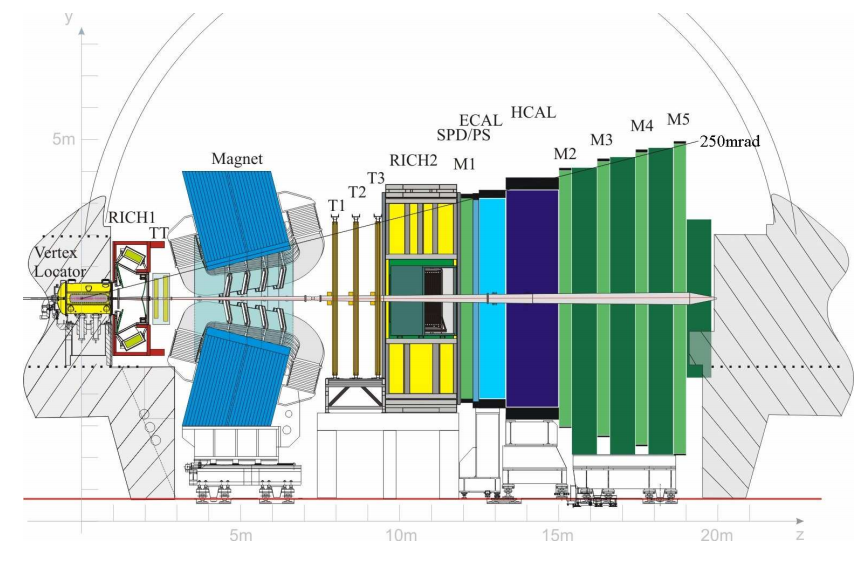
\includegraphics[width=0.8\textwidth]{graphics/lhcb.png}
  \caption{Components of the LHCb detector. \cite{Collaboration_2008}}
  \label{fig:lhcb}
\end{figure}
The LHCb experiment is one of the four main experiments at the Large Hadron Collider (LHC)\cite{Evans_2008} at the nuclear research institute CERN located near Geneva in Switzerland. It is a one-arm forward-spectrometer specifically designed to study \textit{CP} asymmetries as well as rare decays of charm and beauty hadrons. The latter are primaliry produced in gluon fusion processes. The gluons come from the sea of the colliding protons and often have vastly different momentum, resulting in a large Lorentz boost in the beam direction. Therefore charm and beauty hadrons are mostly produced in two cones, motivating the design of the LHCb detector. A schematic of the detector is shown in \autoref{fig:lhcb} and its components are briefly explained in the following.\\

The Vertex Locator (VELO) is a silicon strip detector surrounding the interaction area. It is used for precise measurement of the interaction point as well as the decay vertex, also referred to as secondary vertex, which is destinctive feature for charm and beauty hadron decays. It also collects track data of the charged decay products. Since the VELO is located closer to the beam pipe than required by the LHC during injection it consists of two halves that are retractable.\\

The tracking stations TT, T1, T2 and T3 are silicon microstrip detectors which allow to reconstruct the tracks of charged particles. By measuring the track curvature caused by the magnet the tracking stations can also be used to determine the momentum of the tracked charged particles. To counteract possible detection asymmetries due to the polarity of the magnet it can be operated with either an up or down polarity.\\

The Ring Imaging Cherenkov (RICH) detectors exploit the fact charged particles emit Cherenkov radiation when travelling in a medium with a velocity surpassing that of the speed of light in that medium. The opening angle $\theta$ of the resulting Cherenkov cone is defined as
\begin{equation}
  \cos \theta = \frac{1}{n\beta},
\end{equation}
where $n$ is the refraction index of the medium and $\beta$ is defined as $\beta = \frac{v}{c}$ with the velocity $v$ of the particle and the speed of light in a vacuum $c$. Therefore the RICH detectors can be used to measure the velocity of charged particles. By combining this information with the momentum measured by the tracking system one can infer the mass of the measured particle.\\

The Electromagnetic (ECAL) and Hadronic Calorimeter (HCAL) are the only detector components that are able to measure neutral particles. The calorimeters are composed of material with short radiation length or hadronic interaction length, respectively, so that the particles deposit their total energy. The shower cluster of the deposited energy also allows to infer the particles identity. Besides neutrinos, that cannot be measured by the LHCb detector at all, only muons do not deposit all their energy in the calorimeter system.\\

Muons are minimum ionising particles and hence able to travel through the whole detector. Therefore the muon trackers are, with exception of M1, the last components of the LHCb detector. The muons are identified by a system of iron absorber layers and multi-wire chambers.
